\chapter{Measurement in the dipole trap}
For evaluating the calulations in the experiment the resonance-frequency of the D2-Line was measured. The measurement of the \textsc{ac}-Stark shift is done in the crossed dipole-trap. The magnetic field however was at 527 G for every measurement. To find the resonance peak in the respective setting the atom number is measured using absorption imaging. The frequency of the imaging laser is hereby scanned over the considered resonance, taking 5 images for every step in detuning and taking the average. To find the differential light shift, the pictures are taken either with the activated dipole-trap or with the laser-beams turned off, leaving minimum time of flight in order to get reliable results. The used $D_2$-line corresponds to the transition from  $2s\rightarrow2p_{3/2}$. For technical reasons only the incoming beam of the dipole trap is $\pi$-polarized and the reflected beam has components in \(\sigma^+\) and \(\sigma^-\)-direction. This changes the value for the tensor-polarizability of the excited state but since the trap is far detuned, this component already plays a minor role and the different polarizations should change the overall differential shift only around 0.1 \textsc{mhz}, which cannot be resolved. The initial cloud is a mixture of two spin-species. However, due to the magnetic field the two ground states of $m_J=\pm 1/2$ differ by around 80 MHz due to the Zeeman-effect. Because of the polarization of the imaging laser all excited states would be shifted in the positive direction. While this does not change the behavior of the \textsc{ac}-Stark shift significantly, it does make sure, that only a transition from one ground state is resonant at once. In our case this was the transition: $m_J=+1/2 \rightarrow m_J=+3/2$. 
\begin{figure}[h]
\centering
\begin{subfigure}[b]{0.48\textwidth}
                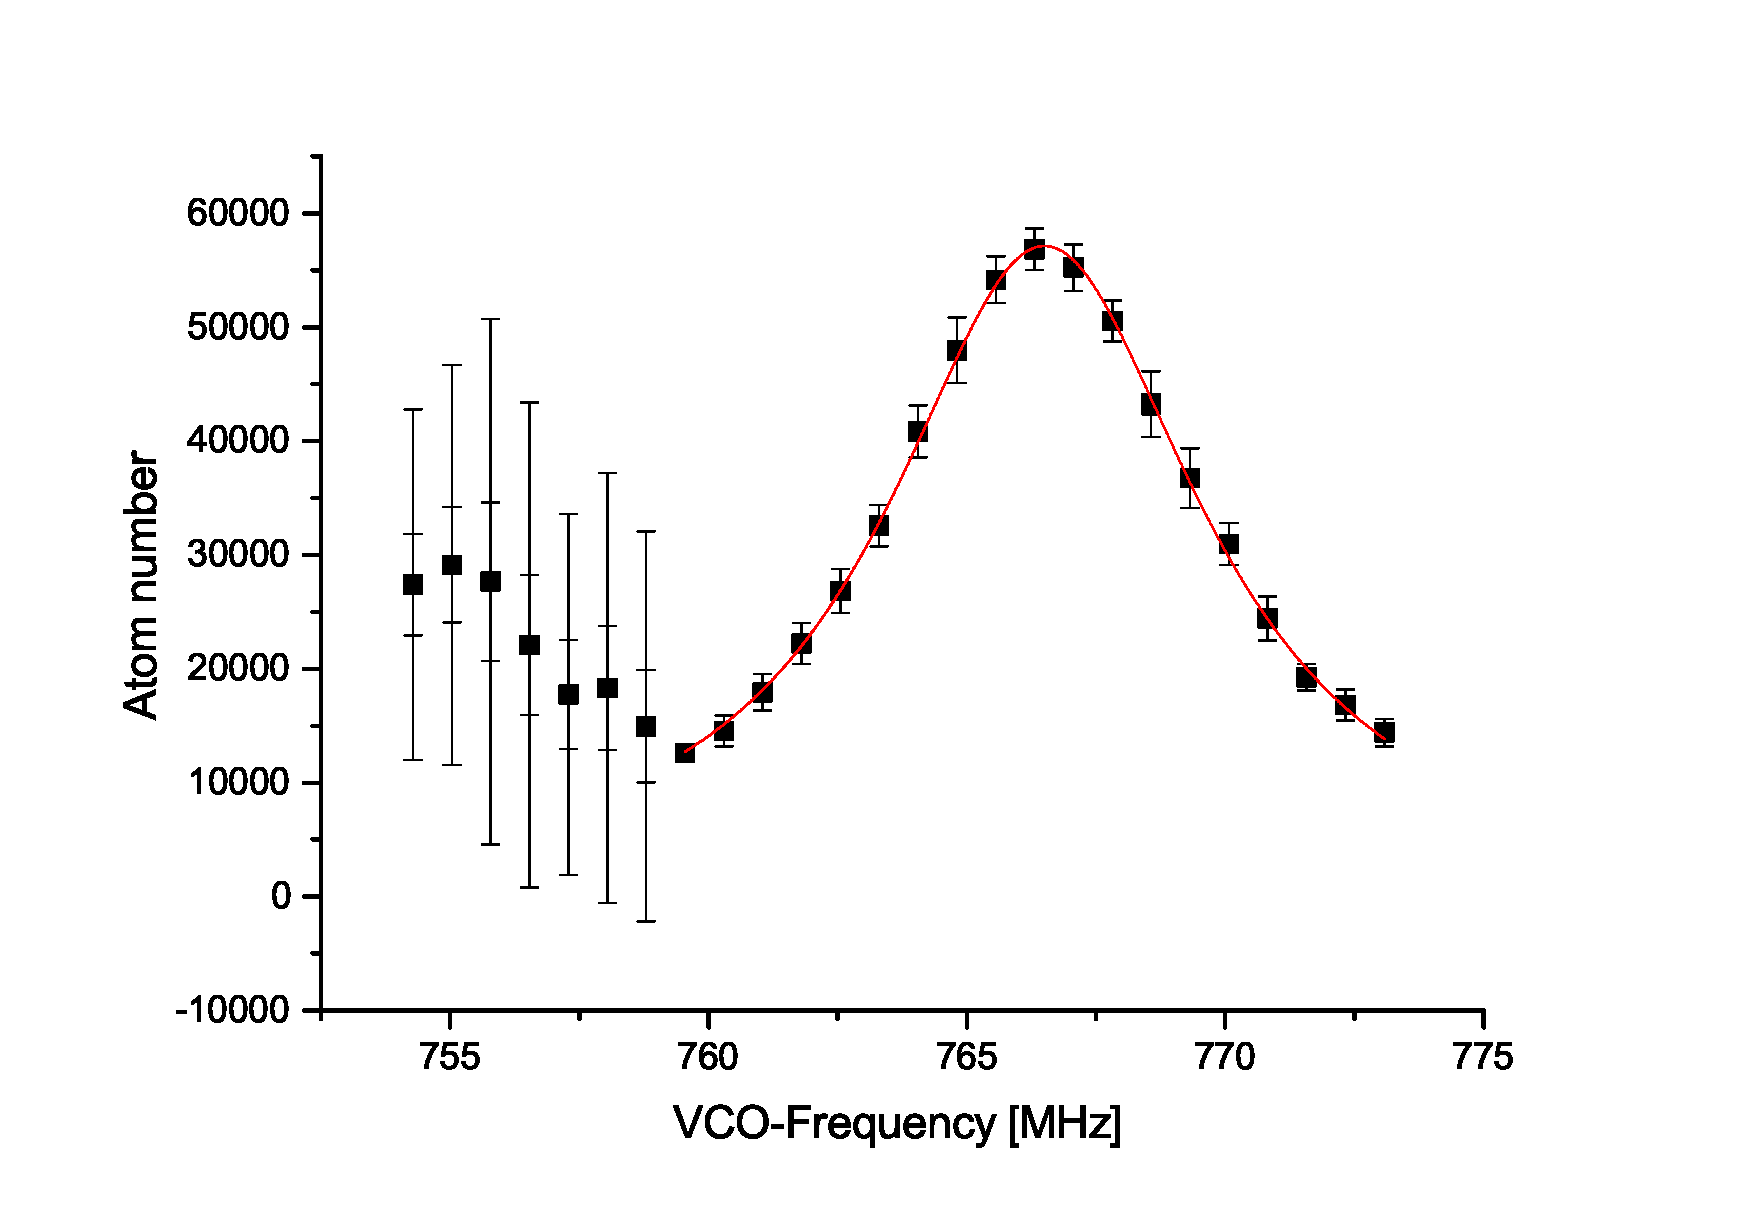
\includegraphics[width=\textwidth]{withoutodt}
                \caption{Dipole-trap turned off.}
\end{subfigure}
\begin{subfigure}[b]{0.48\textwidth}
               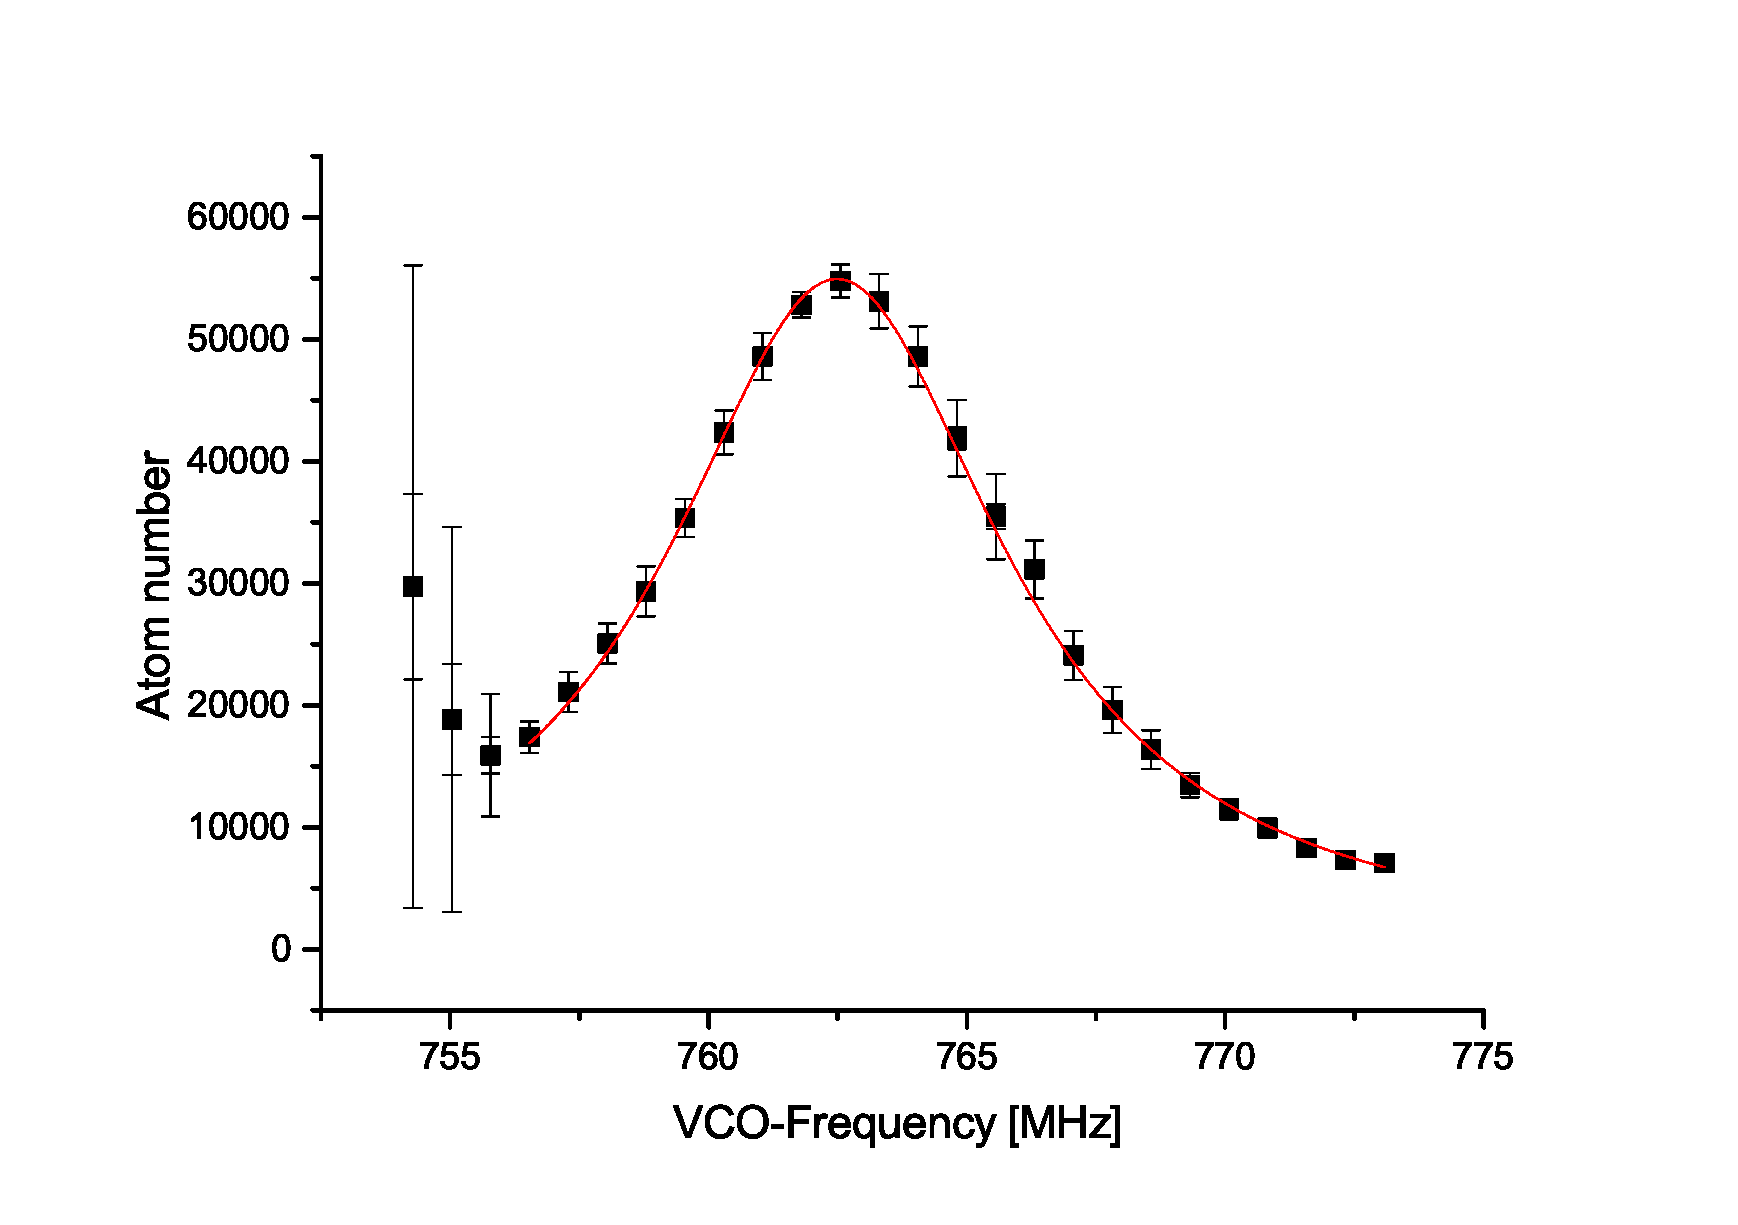
\includegraphics[width=\textwidth]{withodt}
                \caption{Dipole-trap turned on.}
\end{subfigure}


\caption{Resonance peak for the transition: $2s\rightarrow2p_{3/2}, m_j=+3/2$ at 1070 nm. The power at this meassurement was 12.35 W. The scale shows frequencies of the voltrage-controlled oscillator determning the detuning of the laser and is fixed arbitrarily. Also higher frequencies actually mean red detuning. It therefore shows only the relative shift. A Lorentzian function (red) was fitted to the values, whose parameters were used to determine the center position of the peak. In the range, where the laser was effectivly off-resonance the seen atom-cloud lost its gaussian profile, and therefore no fit was possible to determine the atom number. This accounts for the high errors in this range.}
\label{resonance}
\end{figure}	
Since the excited state is expected to be shifted less than the ground state by the \textsc{ac}-Stark shift, the energy difference should increase, leading to a higher resonance frequency and a lower resonance wavelength. The shift is expected to be 0.175\pm 0.060 MHz/W and therefore the resonance frequency for 12.35 W should be 4.3\pm 1.5 MHz lower, when activating the dipoletrap. The resulting graph for this power can be seen in figure \ref{resonance}. To compare the behaviour as well as the exact values with the theory, different powers were measured and plotted in figure \ref{shifts}. 

\begin{figure}[h]
\centering
\begin{subfigure}[b]{0.8\textwidth}
                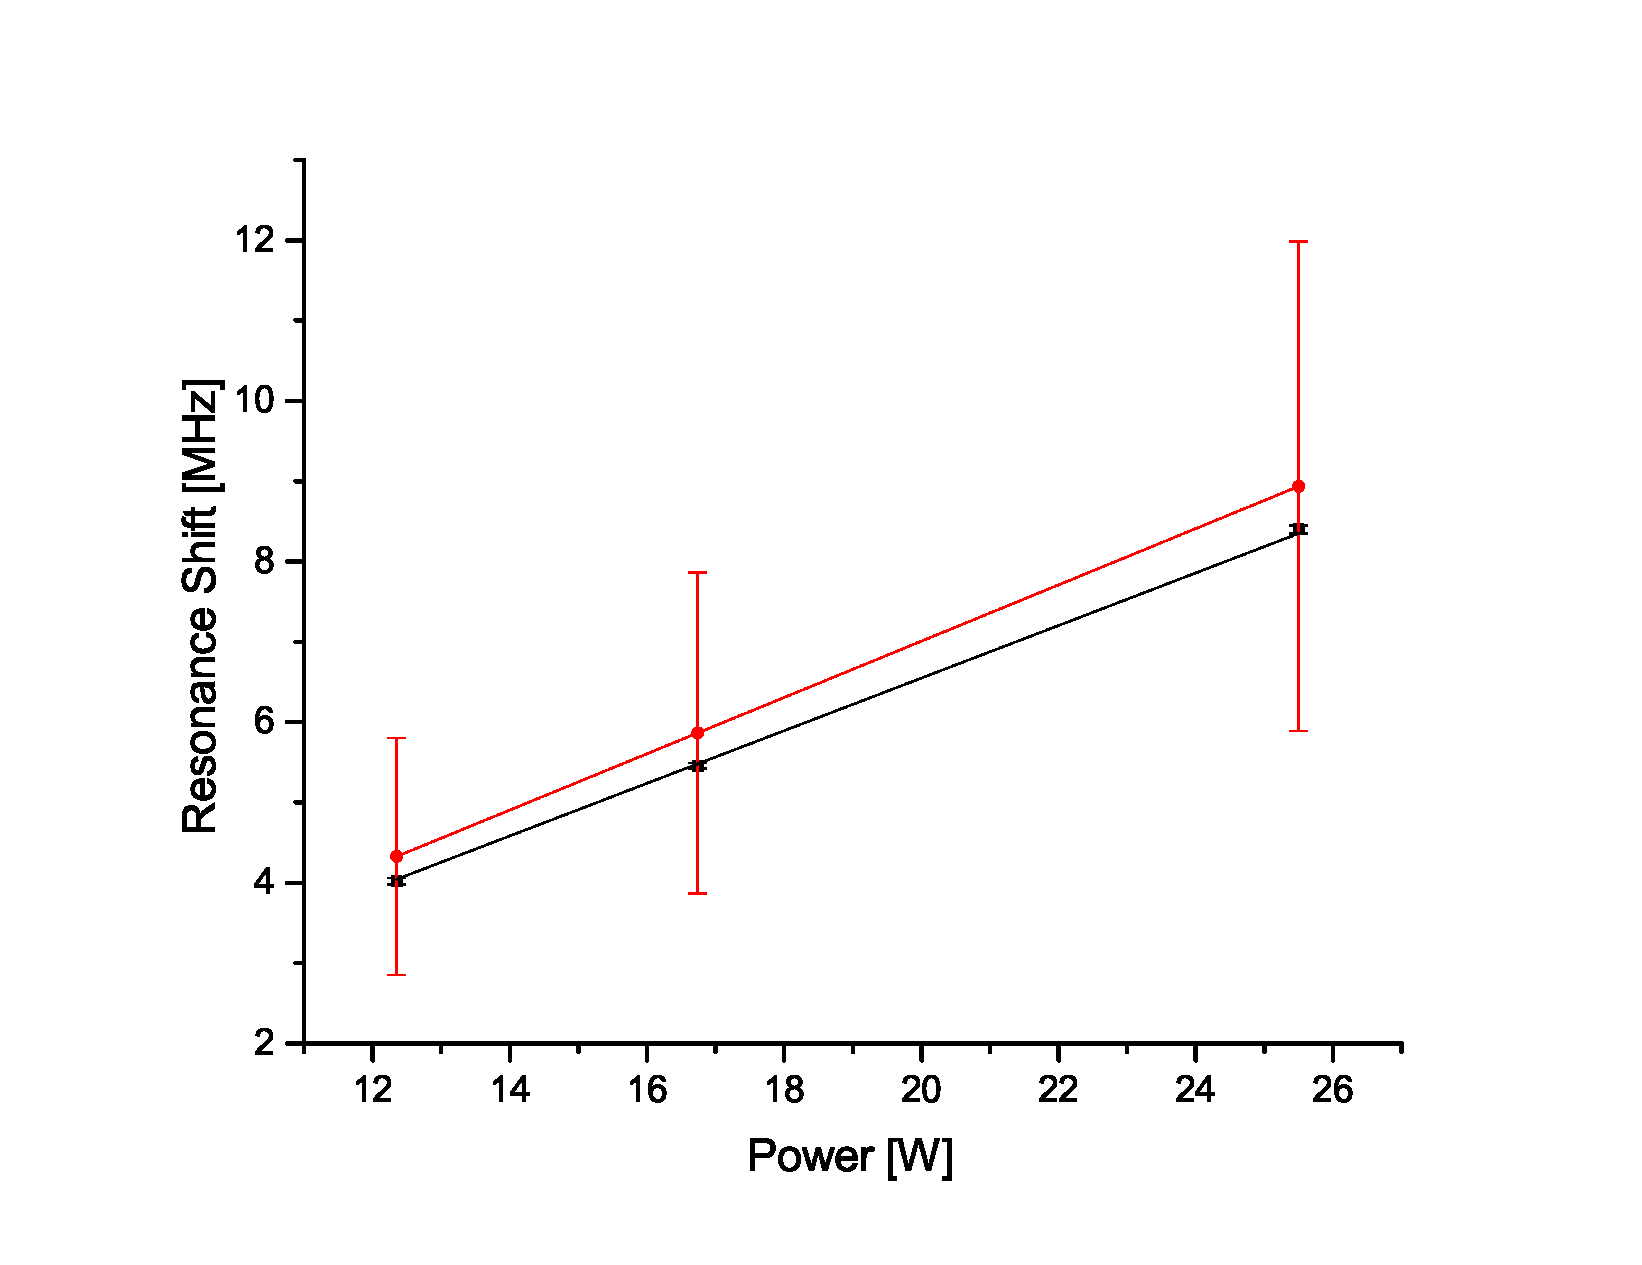
\includegraphics[width=\textwidth]{Shift2}
\end{subfigure}
\caption{Comparison of the differential light-shift in theory (red) and experiment (black) for the D2-line. Note, that the scales show the initial laser powers. The power in the middle of the trap itself is twice as strong. As is visible in this plot, the errors for the measured shifts are very small compared to that of the calculated value. This supports the assumption, that the error is mostly systematic and can be removed in comparison with the measured results.}
\label{shifts}
\end{figure}


As can be seen in figure \ref{shifts} the shifts show a linear behaviour. The fit was fixed at ($P=0, \Delta E_\mathrm{dif}=0$) and still shows a very good  agreement with the prediction. The slope is $0.3274\pm 0.0013\unit{MHz/W}$ of initial beam-power. For a more general statement the value is also given in terms of the intensity:
\begin{figure}[h]
\centering
\begin{subfigure}[b]{0.8\textwidth}
                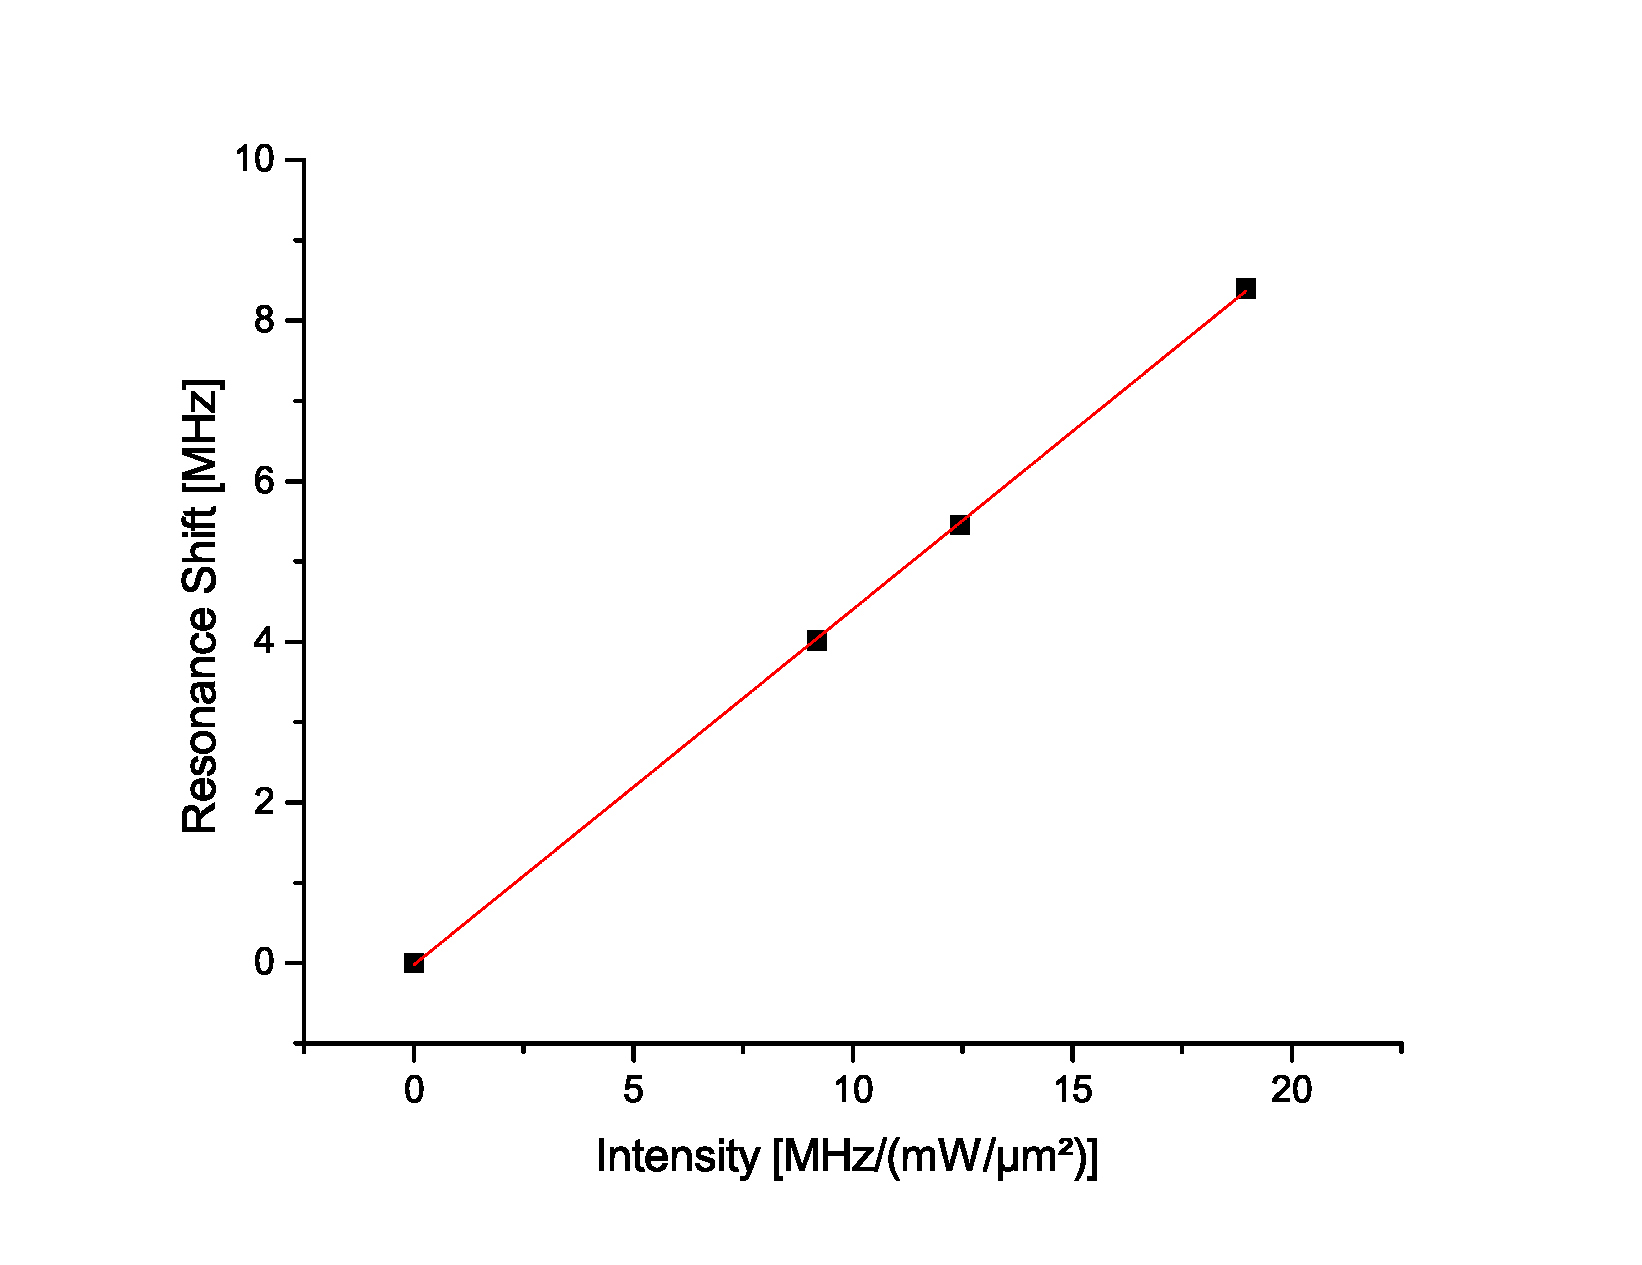
\includegraphics[width=\textwidth]{shiftintens}
\end{subfigure}
\caption{Measured differential shift in terms of intensity.}
\label{shiftintens}
\end{figure}
\begin{equation}
\Delta E_\mathrm{dif}/I=0.4426\pm 0.0028\mathrm{MHz}\frac{1}{\mathrm{mW}/\mu \mathrm{m}^2}
\end{equation}
Using this value, we also can calculate the trap depth, when knowing the relation of both polarizabilities for ground and excited states. The formula is derived using the fact, that the relation between the polarizabilities and thus the light shifts is constant for every power.
\begin{align}
U_{\mathrm{g}}=&-\frac{1}{1-\alpha_{\mathrm{e}}/\alpha_{\mathrm{g}}}\cdot \Delta E_\delta\\
U_{\mathrm{e}}=&-\frac{1}{1-\alpha_{\mathrm{g}}/\alpha_{\mathrm{e}}}\cdot \Delta E_\delta
\end{align}
In this case $\Delta E_\delta$ stands for the relative shift of the levels relative to each other, i.e. the shift of the resonance. The results of the experiment translate into depths of the trap potential for the ground and excited state with the following values:
\begin{align}
U_g/I=&-(120.32\pm 0.48)\ \mu\mathrm{K}\ k_B\frac{1}{\mathrm{mW}/\mu \mathrm{m}^2}\\
U_e/I=&-(78.05\pm 0.31)\ \mu\mathrm{K}\ k_B\frac{1}{\mathrm{mW}/\mu \mathrm{m}^2}
\end{align}
Also the measurement can make it possible to find values for other quantities of the trap. The waist of the trap beam for example is usually not easy to measure exactly, in contrast to its power, that we know with good precision.
\begin{align}
I=&\frac{\epsilon_0 c}{\alpha}\cdot U\\\notag\\
w_0=&\sqrt{\frac{2P}{\pi I}}
\end{align}
In this calculation $I$ is the actual maximum-intensity forming the potential and $P$ the initial laser-power in the trap. For the crossed dipole-trap this results in the following waist.
\begin{equation}
w_0=41.383\pm 0.082 \mu \mathrm{m}
\end{equation}
The approximate value used for the calculation, taken from \cite{lompe} was 40\mu m.

\section{Microtrap parameters}

Using the tested theory we now can calculate the depth for the microtrap. The current waist of the trap is 1.3 $\mu$m using laser power of 400 $\mu$\textsc{w}. This leads to a trap depth of
\begin{align}
U_g=&-(6.03\pm 0.61)\mu\mathrm{K}\ k_B\\
U_e=&-(3.90\pm 0.39)\mu\mathrm{K}\ k_B
\end{align}
Assuming a 5\%-error on the beams waist. We can use $p_\gamma=h/\lambda$ and $T_{Li}=p^2/2m_{Li}$ to calculate recoil energy excited Lithium-6 atom. The trap depth corresponds roughly to the recoil of only a single photon. Therefore the trap is not deep enough for holding an atom for enough absorption events to actually measure the fluorescence. However, it is possible in our setup to ramp the laser power up to about 500 mW, that would correspond to about 1400 photon recoil energies.
\begin{align}
U_g=&-(7.54\pm 0.76)\unit{mK}\ k_B\\
U_e=&-(4.88\pm 0.49)\unit{mK}\ k_B
\end{align}
Taking this as an upper limit in scattered photons before escaping the potential it seems possible to catch enough light of the atoms to detect their fluorescence on the camera. 

